Các thuật toán \eqref{IAPPA1} và \eqref{IAPPA2} sang dạng đơn giản dễ lập trình hơn bằng cách loại bỏ biến \(\nu_k\) và thay thế bằng \(y_k, t_k = 1/\alpha_k\).
Đặt \(a_k = \dfrac{\alpha_k^2}{(1-\alpha_k)A_k\lambda_k} \in [a, 2]\). Thuật toán \eqref{IAPPA2} được rút gọn thành:
\begin{align*}
    t_{k+1} &= \frac{1 + \sqrt{1 + 4(a_k\lambda_k)t_k^2/(a_{k+1}\lambda_{k+1})}}{2}, \\
    x_{k+1} &\approx_2 \operatorname{prox}_{\lambda_k F}(y_k), \\
    y_{k+1} &= x_{k+1} + \frac{t_k - 1}{t_{k+1}}(x_{k+1} - x_k) + (1-a_k)\frac{t_k}{t_{k+1}}(y_k - x_{k+1}).
\end{align*}
\begin{remark}
    Với \(a_k = 2\), khôi phục thuật toán Güler. Tốc độ hội tụ cải thiện khi \(a_k\) nhỏ dần về 0.
\end{remark}
Với \eqref{IAPPA1}, ta có \(a_k = 1\), dạng rút gọn là:
\begin{align*}
    t_{k+1} &= \frac{1 + \sqrt{1 + 4\lambda_k t_k^2/\lambda_{k+1}}}{2}, \\
    x_{k+1} &\approx_1 \operatorname{prox}_{\lambda_k F}(y_k), \\
    y_{k+1} &= x_{k+1} + \frac{t_k - 1}{t_{k+1}}(x_{k+1} - x_k).
\end{align*}
Khi \(\lambda_k\) là hằng số, \eqref{IAPPA1} chính là thuật toán FISTA cổ điển.
\begin{essayonly}
\subsection*{Bài toán thử nghiệm}
Ta xét bài toán hồi quy kiểu LASSO có thêm số hạng "elastic-net":
\begin{equation}
  F(x) = \frac12\norm{Ax-b}^2 + \frac\rho2\norm{x}^2 + \mu\norm{x}_1,
  \qquad x\in\R^n,
  \label{eq:elasticnet}
\end{equation}

với $A\in\R^{m\times n}$, $b\in\R^m$, $\mu,\rho>0$. Đây là hàm lồi {mạnh} (hệ số $\rho$, nhờ số hạng ridge $\rho\norm x^2/2$) -- điều này sẽ cho phép áp dụng trực tiếp Mệnh đề~\ref{prop:relations}(3),
nhưng khi $A$ không phải bội số ma trận đơn vị, toán tử $\prox_{\lambda F}$ {không có công thức đóng}: bài toán con
\[
  \Phi_\lambda(x;y) = \frac12\norm{Ax-b}^2+\frac\rho2\norm x^2
  +\mu\norm x_1+\frac1{2\lambda}\norm{x-y}^2
\]
tự nó là một bài toán tối ưu (tuy lồi mạnh, trơn cộng không trơn) cần được giải bằng một thuật toán con. Đây chính xác là tình huống được nêu
làm động lực trong phần giới thiệu của \citet{salzovilla2012} (khử nhiễu/khử mờ ảnh với biến phân toàn phần, hồi quy thưa có cấu trúc).

Số liệu dùng trong thí nghiệm: $n=80$, $m=30$, vectơ nghiệm thật $x_{\text{true}}$ có $s=8$ thành phần khác 0, $b=Ax_{\text{true}}+$~nhiễu Gauss nhỏ, $\mu=0{,}10$, $\rho=0{,}02$, $\lambda=2$ (hằng số theo $k$, để $M=1$ hiển nhiên đúng).

\subsubsection*{Xây dựng phép xấp xỉ gần kề có kiểm soát}\label{sec:numerical-construction}

Bài toán con $\Phi_\lambda(\cdot;y)$ được giải xấp xỉ bằng
{FISTA nội} (chính thuật toán của \citealp{beck2009fista}, áp
dụng cho phần trơn $\tfrac12\norm{Ax-b}^2+\tfrac\rho2\norm x^2+\tfrac1{2\lambda}\norm{x-y}^2$
và phần không trơn $\mu\norm x_1$, có $\prox$ là phép ngưỡng mềm
\emph{soft-thresholding}). Cho $T$ lần lặp nội, gọi $z_T$ điểm lặp thứ
$T$. Hai bước sau đây biến $z_T$ thành một {chứng nhận toán học
đầy đủ}, không phải một xấp xỉ "chấp nhận được về mặt trực giác":

\begin{enumerate}[leftmargin=1.6em]
  \item \textbf{Loại 1.} Theo chính đẳng thức
  \eqref{eq:eps-subopt} áp dụng cho $\Phi_\lambda$: nếu ta đo được (hoặc
  chặn trên được) độ lệch hàm mục tiêu nội
  $\delta_{\text{inner}} := \Phi_\lambda(z_T;y)-\Phi_\lambda^*(y)$, thì
  $z_T$ {tự động} là một xấp xỉ loại 1 của $\prox_{\lambda F}(y)$
  với độ chính xác
  \[
    \eps^{(1)} = \sqrt{2\lambda\,\delta_{\text{inner}}}.
  \]
  Trong cài đặt, $\Phi_\lambda^*(y)$ (không biết chính xác) được ước lượng bởi giá trị nhỏ nhất trong toàn bộ vết $T_{\text{ref}}=200$
  lần lặp nội (một mốc gần-đúng-tuyệt-đối, xem mã nguồn
  \texttt{inner\_fista\_trace.m}).
  \item \textbf{Loại 2.} Vì $F$ ở \eqref{eq:elasticnet} lồi
  mạnh hệ số $\rho$, Mệnh đề~\ref{prop:relations} (3) cho phép suy ra {ngay lập tức}, từ cùng một điểm $z_T$, một chứng nhận xấp xỉ loại 2 với độ chính xác
  \[
    \eps^{(2)} = \eps^{(1)}\sqrt{\frac{\lambda\rho+1}{\lambda\rho}}.
  \]
\end{enumerate}

Nói cách khác: {chỉ một} lần giải gần đúng bài toán con, ta thu được đồng thời hai chứng nhận sai số hợp lệ (loại 1 và loại 2) cho cùng một điểm -- và có thể đưa cùng quỹ đạo $(x_k)$ đi qua cả hai bộ sổ sách kế toán $(\eta_k,\delta_k)$ của IAPPA1 và $(\delta_k)$ của IAPPA2 để so sánh trực tiếp hai chặn lý thuyết trên cùng dữ liệu thực nghiệm.
Toán tử ngưỡng mềm và bộ giải FISTA nội:

\begin{lstlisting}[language=Matlab, caption={Toán tử prox của $\ell_1$ (tệp \texttt{soft\_threshold.m}).}]
function x = soft_threshold(v, tau)
x = sign(v) .* max(abs(v) - tau, 0);
end
\end{lstlisting}

\lstinputlisting[language=Matlab, firstline=4,
  caption={Bộ giải FISTA nội, trả về toàn bộ vết lặp (tệp \texttt{code/matlab/inner\_fista\_trace.m}).}]
  {code/matlab/inner_fista_trace.m}

\lstinputlisting[language=Matlab, firstline=18, lastline=47,
  caption={Vòng lặp ngoài chính (trích từ \texttt{code/matlab/run\_outer.m}).}]
  {code/matlab/run_outer.m}
\begin{figure}[H]
    \centering
    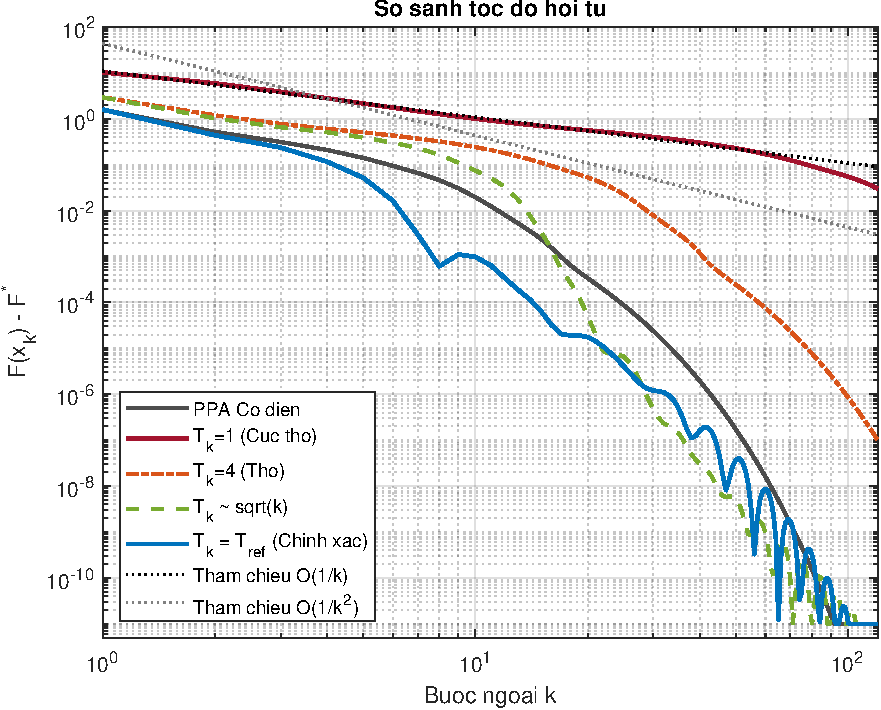
\includegraphics[width=0.8\linewidth]{figures/convergence-comparison.pdf}
    \caption{So sánh tốc độ hội tụ của thuật toán PPA cổ điển và các biến thể ứng với các lịch trình \(T_k\) khác nhau. Kết quả thực nghiệm cho thấy lịch trình \(T_k \sim \sqrt{k}\) duy trì tốc độ hội tụ \(O(1/k^2)\), gần như tương đương với trường hợp giải chính xác (\(T_k = T_{\mathrm{ref}}\)), đồng thời giúp giảm đáng kể chi phí tính toán.}
    \label{fig:conv-comparison}
\end{figure}
\begin{figure}[H]
    \centering
    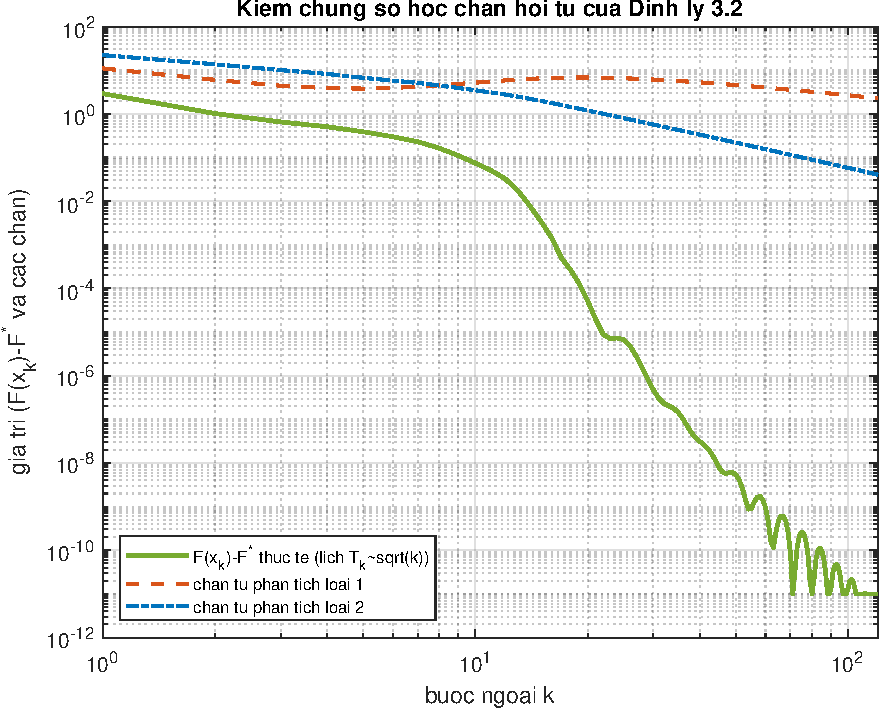
\includegraphics[width=0.8\linewidth]{figures/bound-verification.pdf}
    \caption{Kiểm chứng số học các chặn hội tụ của Định lý~\ref{thm:estimate-main}. Đồ thị log-log biểu diễn khoảng cách của hàm mục tiêu $F(x_k) - F^*$ (đường liền nét màu xanh lá) theo các bước lặp ngoài $k$, được so sánh với chặn lý thuyết Loại 1 (đường đứt nét màu cam) và chặn lý thuyết Loại 2 (đường gạch chấm màu xanh dương). Kết quả thực nghiệm cho thấy với lịch trình vòng lặp nội $T_k \approx \sqrt{k}$, thuật toán hội tụ nhanh hơn và chặt chẽ hơn nhiều so với dự đoán của các giới hạn lý thuyết, và đi ngang ở ngưỡng $10^{-11}$ do giới hạn độ chính xác của máy tính (sàn nhiễu).}
    \label{fig:bound-verification}
\end{figure}
\begin{figure}[H]
    \centering
    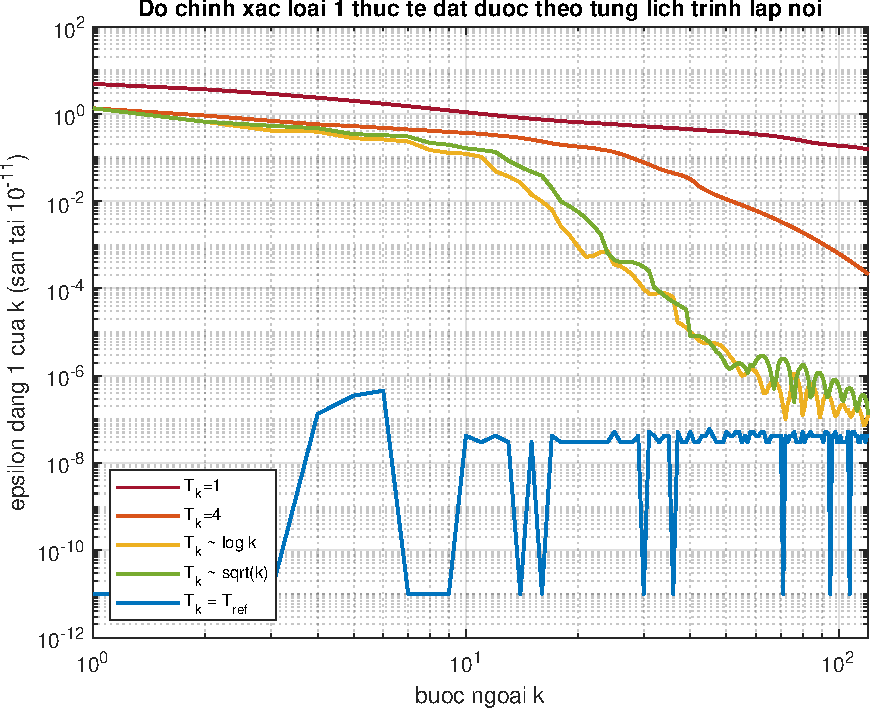
\includegraphics[width=0.8\linewidth]{figures/type1-accuracy.pdf}
    \caption{Sự suy giảm của sai số Loại 1 ($\epsilon_k$) theo số bước lặp ngoài $k$ dưới các kịch bản chọn số vòng lặp nội $T_k$ khác nhau. Biểu đồ log-log cho thấy các chiến lược tăng dần $T_k$ theo bước lặp, cụ thể là $T_k \sim \log k$ (đường màu vàng) và $T_k \sim \sqrt{k}$ (đường màu xanh lá), giúp sai số hội tụ nhanh chóng và đạt hiệu quả cao. Ngược lại, việc cố định $T_k$ ở mức thấp ($T_k=1$ hoặc $T_k=4$) khiến sai số giảm rất chậm. Lịch trình tính toán gần đúng chính xác ($T_k = T_{ref}$, đường màu xanh dương) nhanh chóng dao động quanh mức giới hạn sàn nhiễu số học của máy tính ($10^{-11}$).}
    \label{fig:eps-decay}
\end{figure}
\end{essayonly}
\begin{slidesonly}
    \begin{figure}[H]
    \centering
    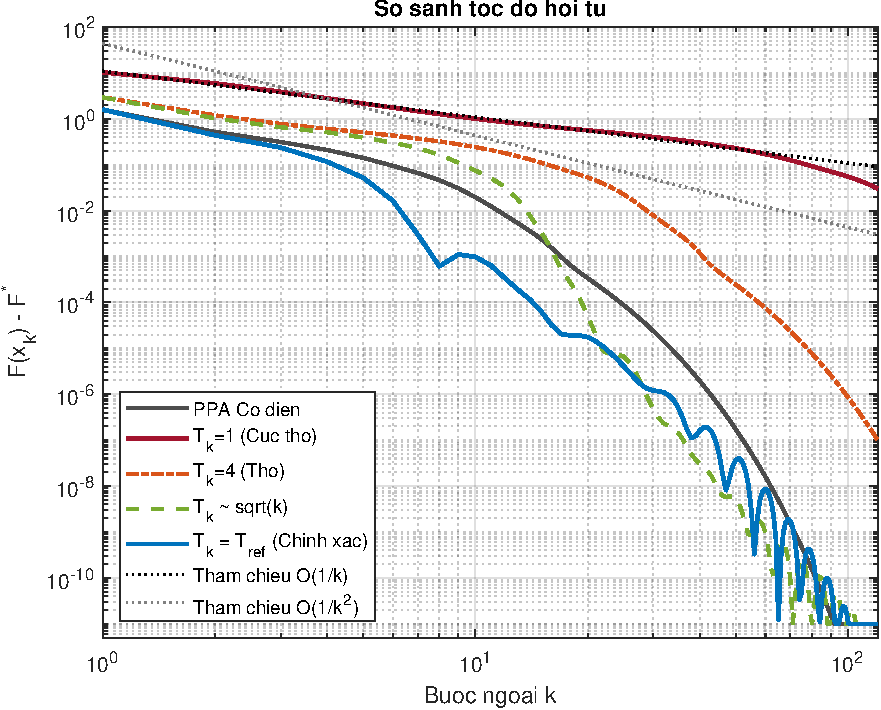
\includegraphics[width=0.9\textwidth, height=0.9\textheight, keepaspectratio]{figures/convergence-comparison.pdf}
    \label{fig:conv-comparison-slide}
\end{figure}
\end{slidesonly}